{一棵m阶B树是一棵平衡的m叉查找树,深度为m。它或者是空树,或者是满足下列性质的树:}

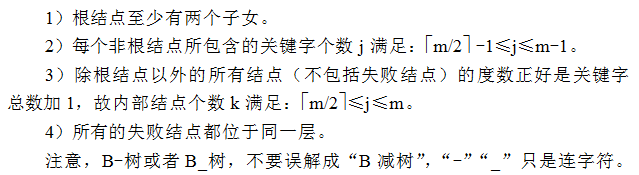
\includegraphics[width=3.70833in,height=1.01042in]{png-jpeg-pics/8B9FFB1654B52E5281DEEC31E5542D98.png}

{\\
}

{\textbf{1. B-树的查找}}

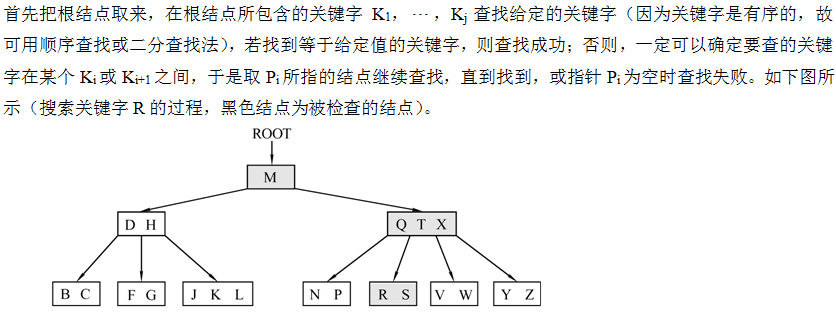
\includegraphics[width=3.70833in,height=1.39583in]{png-jpeg-pics/C68BFA227408F8456869E5A3ECA063AA.png}

{}

{ }

{\textbf{2. B-树的插入}}

{对于关键字的插入,需要找到插入位置。在B-树的查找过程中,当遇到空指针则证明查找不成功,同时也找到了插入位置,即根据空指针可以确定在叶结点中的插入位置。B-树的插入总是发生在叶子结点上。在插入过程中有可能破坏B-树的特性,比如新关键字插入使得结点中关键字的个数超出规定个数,这时要进行结点的拆分。}

{\textbf{3. B-树的删除}}

{\textbf{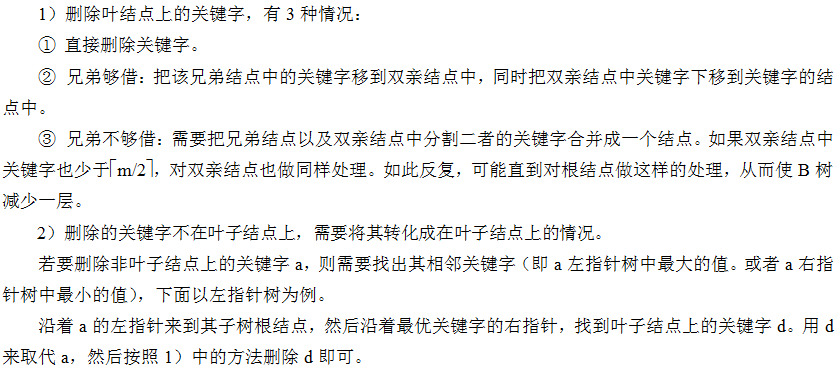
\includegraphics[width=3.70833in,height=1.64583in]{png-jpeg-pics/61618BE80845AD4A7A536F8ADE89229F.png}\\
}}
